% Tikz File 'topology_general.tex'
\documentclass{standalone}
\usepackage[dvipsnames]{xcolor}
\usepackage{tikz,amsmath,amssymb}
\usetikzlibrary{arrows,snakes,backgrounds}
    \begin{document}
    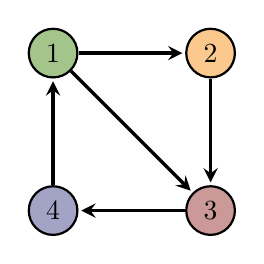
\begin{tikzpicture}[->,shorten >=1pt,auto,semithick]
        \tikzstyle{admmnode}=[
            circle,
            draw=black,
            thick,
            fill=gray,
            text=black
        ]
        \tikzstyle{centernode}=[
            diamond,
            draw=black,
            thick,
            fill=gray!40,
            text=black
        ]

        \node[admmnode, fill=OliveGreen!40] (A) at (-1,1){\(1\)};
        \node[admmnode, fill=BurntOrange!40] (B) at (1,1){\(2\)};
        \node[admmnode, fill=Maroon!40] (C) at (1,-1){\(3\)};
        \node[admmnode, fill=MidnightBlue!40] (D) at (-1,-1){\(4\)};
        % \node[centernode] (F) at (0,0){\(C\)};
        
        \draw[-stealth, line width=1.25] (A) to[bend left=0] node[]{}  (B);
        \draw[-stealth, line width=1.25] (A) to[bend left=0] node[]{} (C);
        \draw[-stealth, line width=1.25] (B) to[bend left=0] node[]{} (C);
        \draw[-stealth, line width=1.25] (C) to[bend left=0] node[]{} (D);
        \draw[-stealth, line width=1.25] (D) to[bend left=0] node[]{} (A);
        % \draw[stealth-stealth, line width=1.25, draw=gray] (A) to[bend left=0] node[]{} (F);
        % \draw[stealth-stealth, line width=1.25, draw=gray] (B) to[bend left=0] node[]{} (F);
        % \draw[stealth-stealth, line width=1.25, draw=gray] (C) to[bend left=0] node[]{} (F);
        % \draw[stealth-stealth, line width=1.25, draw=gray] (D) to[bend left=0] node[]{} (F);
        
    \end{tikzpicture}
\end{document}